%%%%%%%%%%%%%%%%%%%%%%%%%%%%%%%%%%%%%%%%%%%%%%%%%%%%%%%%%%%%%%%%%%%%%%%%%%%%%
% 26/05/2010
% edited by Bill Lampos
%
% Feel free to use (copy) the structure (latex formatting source code)
% but not the content of this document.
%
%%%%%%%%%%%%%%%%%%%%%%%%%%%%%%%%%%%%%%%%%%%%%%%%%%%%%%%%%%%%%%%%%%%%%%%%%%%%%
\documentclass[compress,blue]{beamer}
\usepackage{etex}
\mode<presentation>

\usetheme{Warsaw}
% other themes: AnnArbor, Antibes, Bergen, Berkeley, Berlin, Boadilla, boxes, CambridgeUS, Copenhagen, Darmstadt, default, Dresden, Frankfurt, Goettingen,
% Hannover, Ilmenau, JuanLesPins, Luebeck, Madrid, Maloe, Marburg, Montpellier, PaloAlto, Pittsburg, Rochester, Singapore, Szeged, classic

%\usecolortheme{lily}
% color themes: albatross, beaver, beetle, crane, default, dolphin, dov, fly, lily, orchid, rose, seagull, seahorse, sidebartab, structure, whale, wolverine

%\usefonttheme{serif}
% font themes: default, professionalfonts, serif, structurebold, structureitalicserif, structuresmallcapsserif

% pdf is displayed in full screen mode automatically
%\hypersetup{pdfpagemode=FullScreen}

% define your own colours:
\definecolor{Red}{rgb}{1,0,0}
\definecolor{Blue}{rgb}{0,0,1}
\definecolor{Green}{rgb}{0,1,0}
\definecolor{magenta}{rgb}{1,0,.6}
\definecolor{lightblue}{rgb}{0,.5,1}
\definecolor{lightpurple}{rgb}{.6,.4,1}
\definecolor{gold}{rgb}{.6,.5,0}
\definecolor{orange}{rgb}{1,0.4,0}
\definecolor{hotpink}{rgb}{1,0,0.5}
\definecolor{newcolor2}{rgb}{.5,.3,.5}
\definecolor{newcolor}{rgb}{0,.3,1}
\definecolor{newcolor3}{rgb}{1,0,.35}
\definecolor{darkgreen1}{rgb}{0, .35, 0}
\definecolor{darkgreen}{rgb}{0, .6, 0}
\definecolor{darkred}{rgb}{.75,0,0}

\xdefinecolor{olive}{cmyk}{0.64,0,0.95,0.4}
\xdefinecolor{purpleish}{cmyk}{0.75,0.75,0,0}

% \usepackage{beamerinnertheme_______}
% inner themes include circles, default, inmargin, rectangles, rounded

%\usepackage{beamerouterthemesmoothbars}
% outer themes include default, infolines, miniframes, shadow, sidebar, smoothbars, smoothtree, split, tree

\useoutertheme[subsection=false]{smoothbars}

% to have the same footer on all slides
%\setbeamertemplate{footline}[text line]{xxx xxx xxx}
%\setbeamertemplate{footline}[text line]{} % or empty footer

% include packages
\usepackage{subfigure}
\usepackage{multicol}
\usepackage{amsmath}
\usepackage{epsfig}
\usepackage{helvet}
\usepackage{graphicx}
\usepackage[all,knot]{xy}
\xyoption{arc}
\usepackage{url}
\usepackage{multimedia}
\usepackage{hyperref}
\usepackage{setspace}

\title{Agents Interaction}
\subtitle{and the Predators-Prey Model}
\author{Ali Saleh}
\institute{{\tiny advised by}\\ \vspace{.10cm}Prof. Dr. Andreas G. Fleischer}
\date{\scriptsize Universit\"{a}t Hamburg \\ \vspace{.10cm}Jan 21, 2015}

\begin{document}

\frame{
	\titlepage
}

\section[Outline]{}
\frame{\tableofcontents}

\section{Introduction to Predator-prey model}
\subsection{General Model}
\frame{\frametitle{General Model}
First studied independently by 2 mathematicians Lotka \& Volterra in the 1920s.
\vspace{0.15cm}
\begin{itemize}
\item Describes the evolution of competing species in an eco-system.
\vspace{0.15cm}
\item Formulated as a nonlinear system of differential equations.
\vspace{0.15cm}
\item Several more sophisticated models have been developed to discuss more details.
\vspace{0.15cm}
\item Model have been adapted in other fields (e.g. Goodwin model for economics)
\end{itemize}
}

\frame{\frametitle{General Model Cont.}
\begin{figure}[hbtp]
\centering
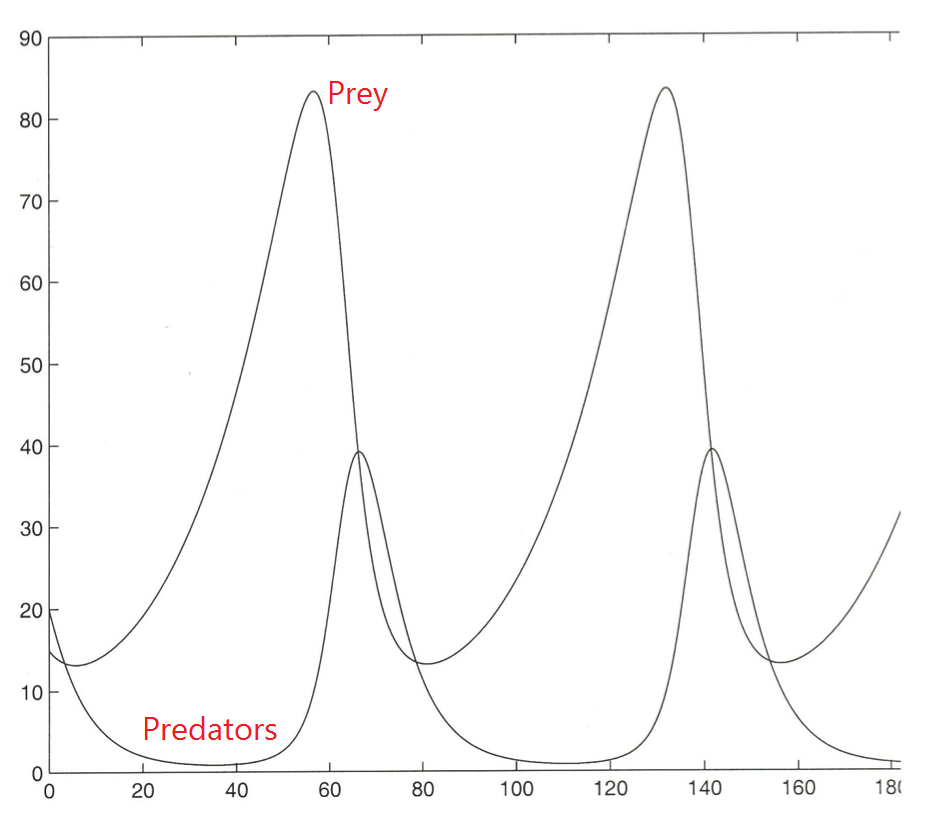
\includegraphics[width=190pt,height=180pt]{figures/graph11.png}
\caption{\scriptsize Periodic activity predicted by the Predator-Prey model. [1]}
\end{figure}

}

\subsection{Limitations of the Mathematical Models}
\frame{\frametitle{Limitations of the Mathematical Models}
While the mathematical models are a very powerful tool to describe 
the behavior of the system, it also have it's limitations
\vspace{0.25cm}
\begin{itemize}
   \item Cannot catch the interactions between individuals \vspace{0.15cm}
   \vspace{0.15cm}
   \item Harder for non-mathematicians to understand \vspace{0.15cm}
   \vspace{0.15cm}
   \item Not easy to visualize the different states of the system. \vspace{0.15cm}
\end{itemize}
}

\section{Cellular Automaton Evolution}
\subsection{Cellular Automaton}
\frame{\frametitle{Cellular Automaton}
Grid of cells used in studying evolution of models
\vspace{0.15cm}
\begin{itemize}
\item Finite dimensions \vspace{0.15cm}
\item Discrete time steps \vspace{0.15cm}
\item Finite States \vspace{0.15cm}
\item New states from old state generated by fixed rules \vspace{0.15cm}
\item example : Conway's Game of Life \vspace{0.15cm}
\end{itemize}
}

\subsection{Simple Predator-Prey CA}
\frame{\frametitle{Predator-Prey CA}
The Simple Cellular Automaton simulation for the predator-prey model had some assumption
\begin{itemize}
\item Closed system (no migration allowed) \vspace{0.15cm}
\item 2 dimensional grid \vspace{0.15cm}
\item Only 2 types of agents/animals (Predators \& Preys) \vspace{0.15cm}
\item Birth rate for preys 99.5\% \vspace{0.15cm}
\item Birth rate for predators 75\% \vspace{0.15cm}
\end{itemize}
}

\frame{\frametitle{Predator-Prey CA}
\begin{figure}[hbtp]
\centering
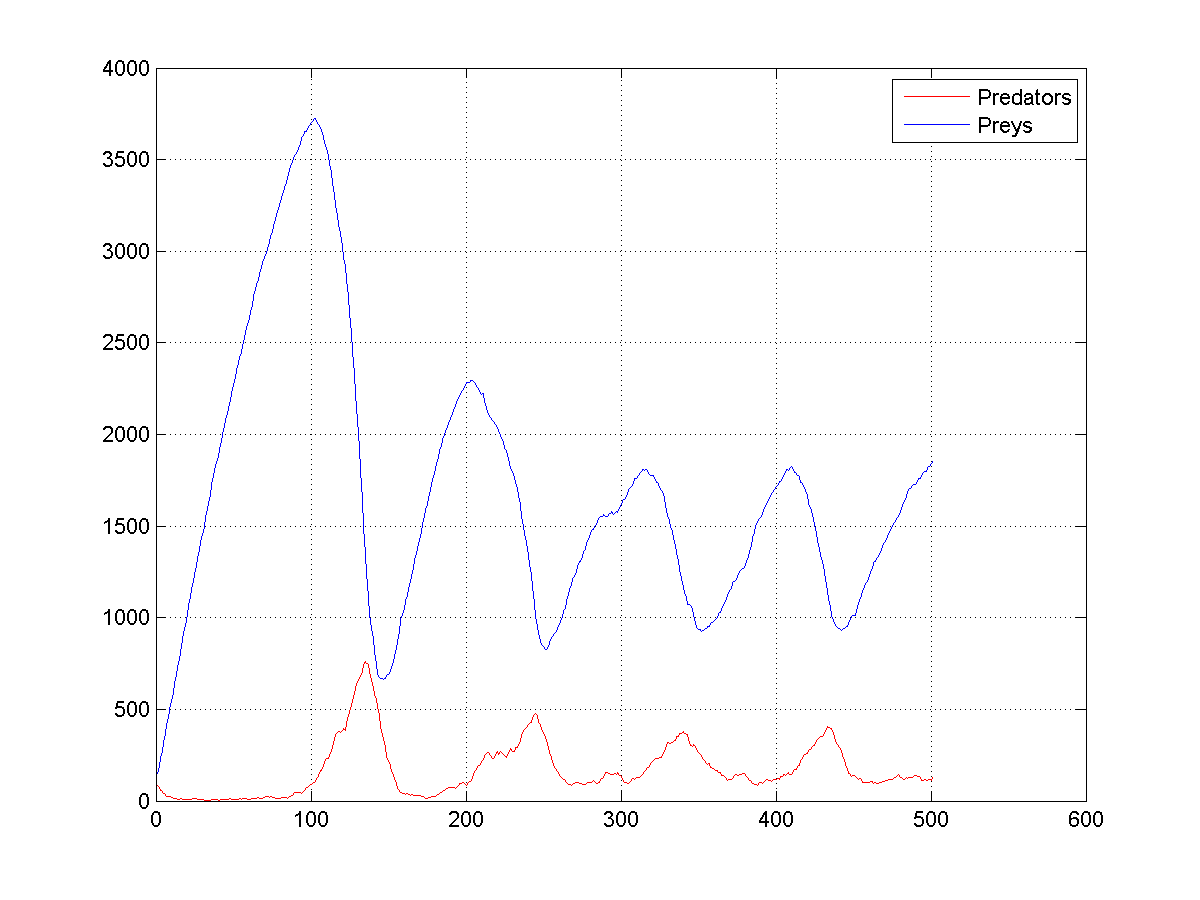
\includegraphics[width=250pt,height=220pt]{figures/simpleImage.png}
\caption{Predators vs Preys population through time}
\end{figure}
}

\frame{\frametitle{Predator-Prey CA}
\begin{figure}[hbtp]
\centering
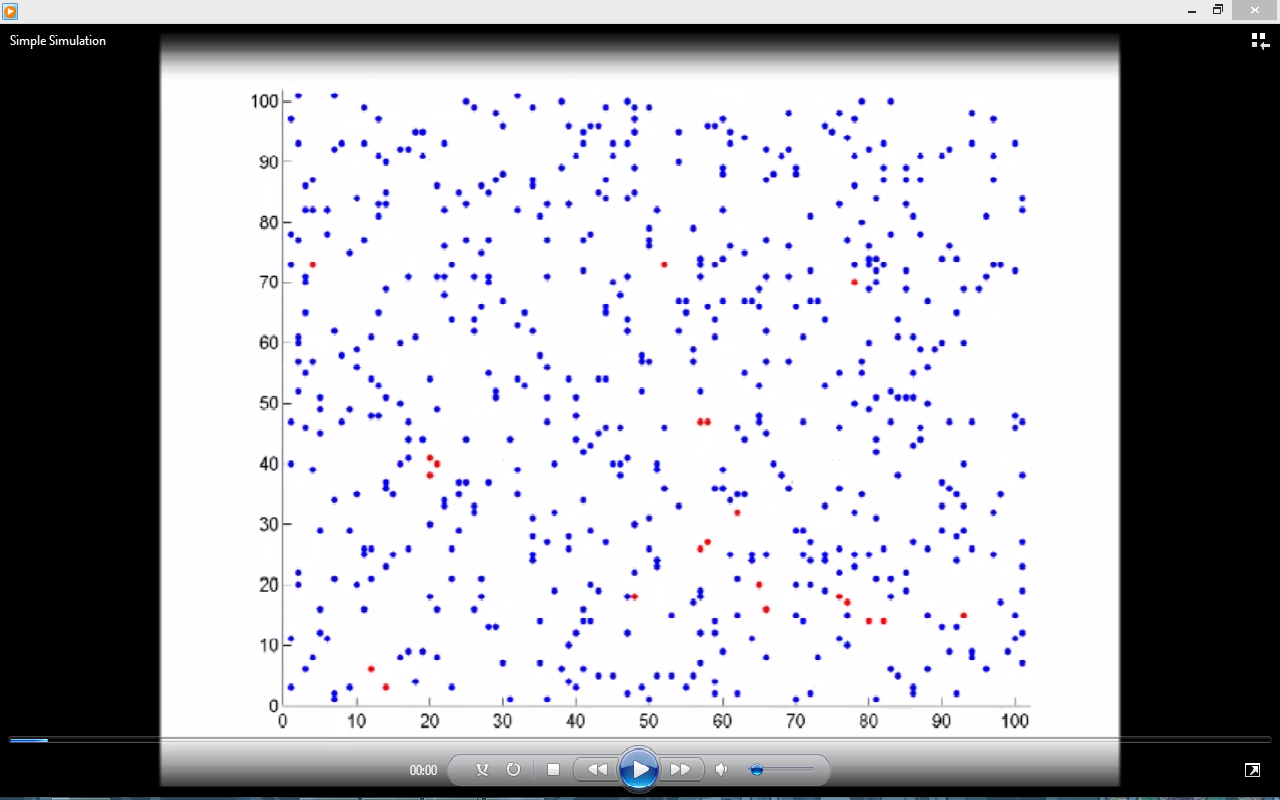
\includegraphics[width=250pt,height=190pt]{figures/simpleVideo.png}
\end{figure}
}

\section{The Effect of Niches}
\frame{\frametitle{The Effect of Niches}
In this section two variations of the simple CA are examined
\begin{itemize}
\item Manipulating the CA to have an area where the Predators cannot enter
\item Manipulating the CA to have 2 levels of predators birth rate
\end{itemize}
}

\subsection{No-Predator Area}
\frame{\frametitle{No-Predator Area}
This simulation is characterized as following
\begin{itemize}
\item A square in the middle that Predators cannot enter (i.e. Niche)
\item The Preys birth rate in the Niche is 99.5\%
\item The Preys birth rate outside the Niche is 99\%
\item The Predators birth rate outside the Niche is 75\%
\item If the density of Preys in the Niche is over 90\% , then 20\% of the 
population will die from over population
\end{itemize}
}

\frame{\frametitle{No-Predator Area}
\begin{figure}[hbtp]
\centering
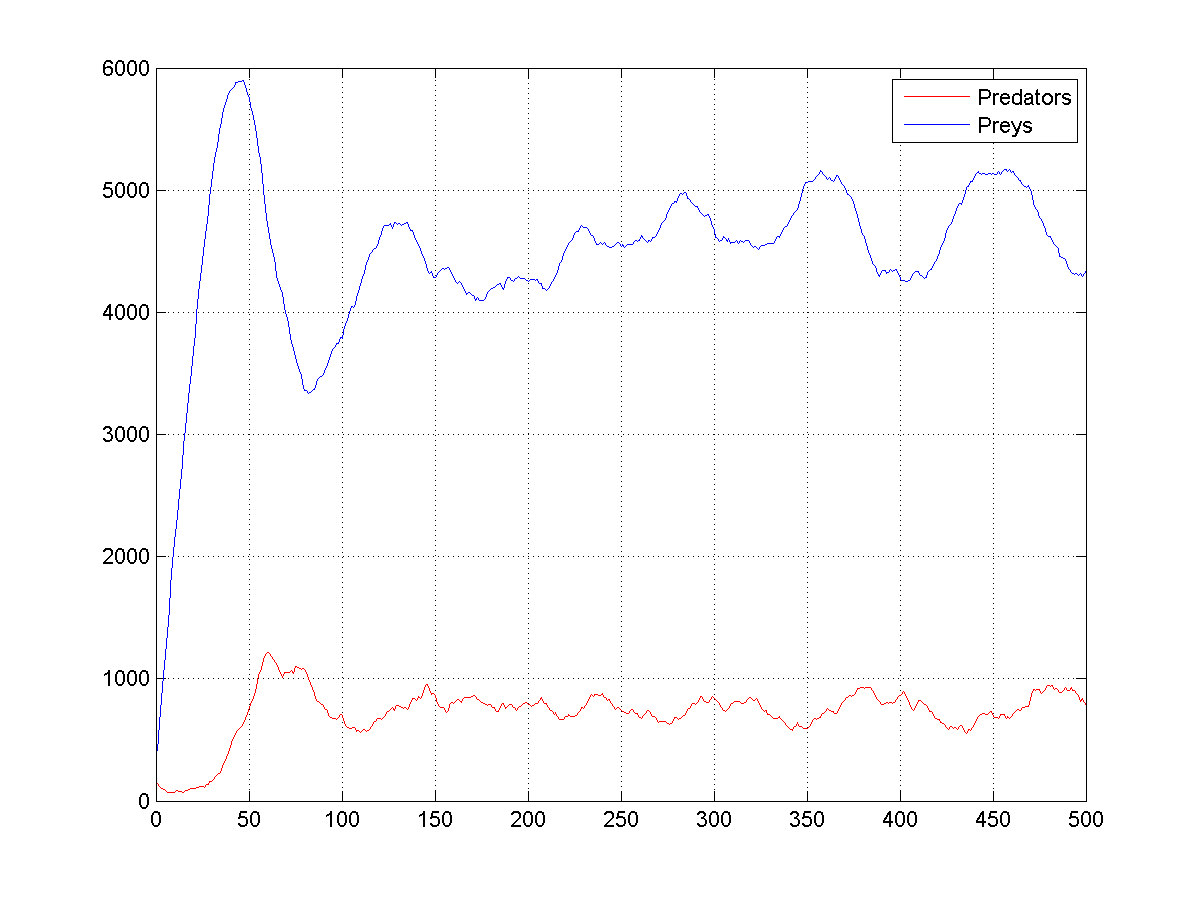
\includegraphics[width=250pt,height=220pt]{figures/NicheImage.png}
\caption{Predators vs Preys population through time}
\end{figure}
}

\frame{\frametitle{No-Predator Area}
\begin{figure}[hbtp]
\centering
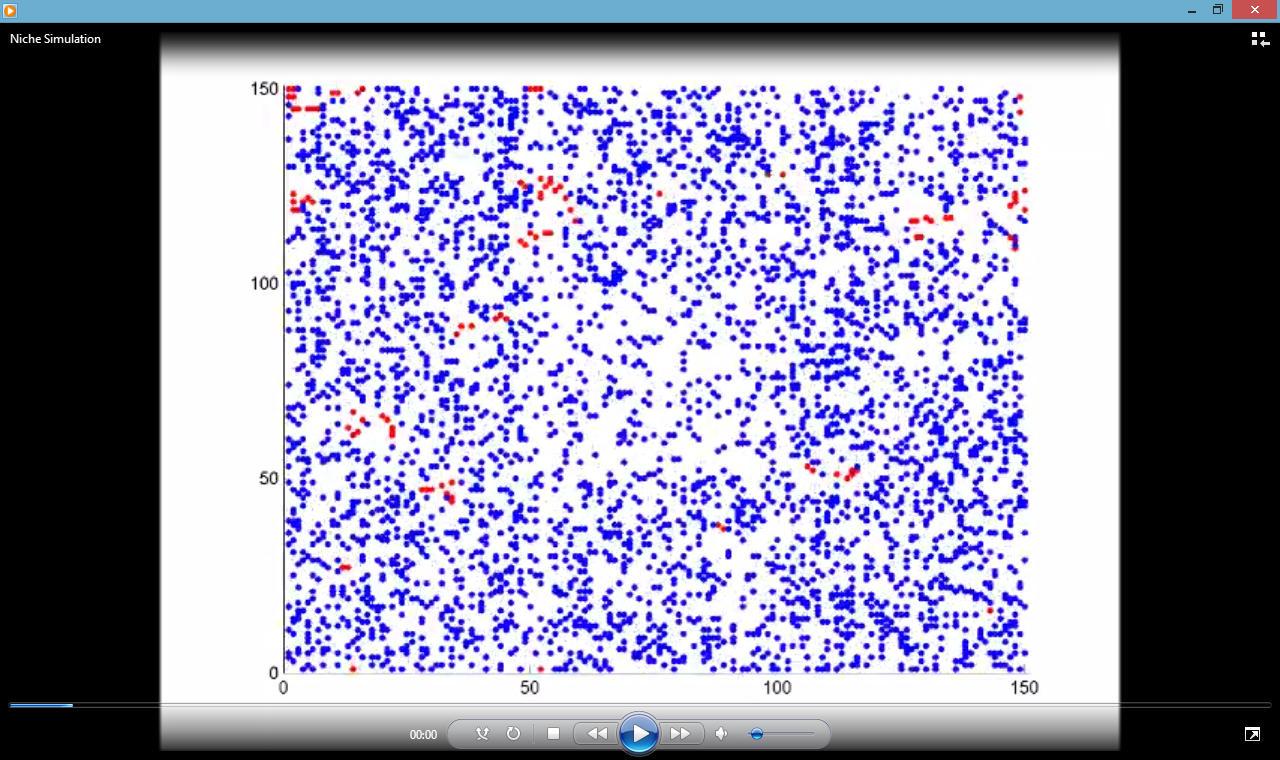
\includegraphics[width=250pt,height=190pt]{figures/NicheVideo.png}
\end{figure}
}

\subsection{2 Levels Niche}
\frame{\frametitle{2 Levels Niche}
This simulation is characterized as following
\begin{itemize}
\item A Niche with the same properties as previous section
\item The area outside the Niche is divided into two levels
\begin{enumerate}
\item Area 1 The Square enclosing the Niche with Preys birth rate 99\% \& Predators Birth rate 75/%
\item Area 2 The Outer Square enclosing the Niche with Preys birth rate 95\% \& Predators Birth rate 80/%
\end{enumerate}

\end{itemize}
}

\frame{\frametitle{2 Levels Niche}
\begin{figure}[hbtp]
\centering
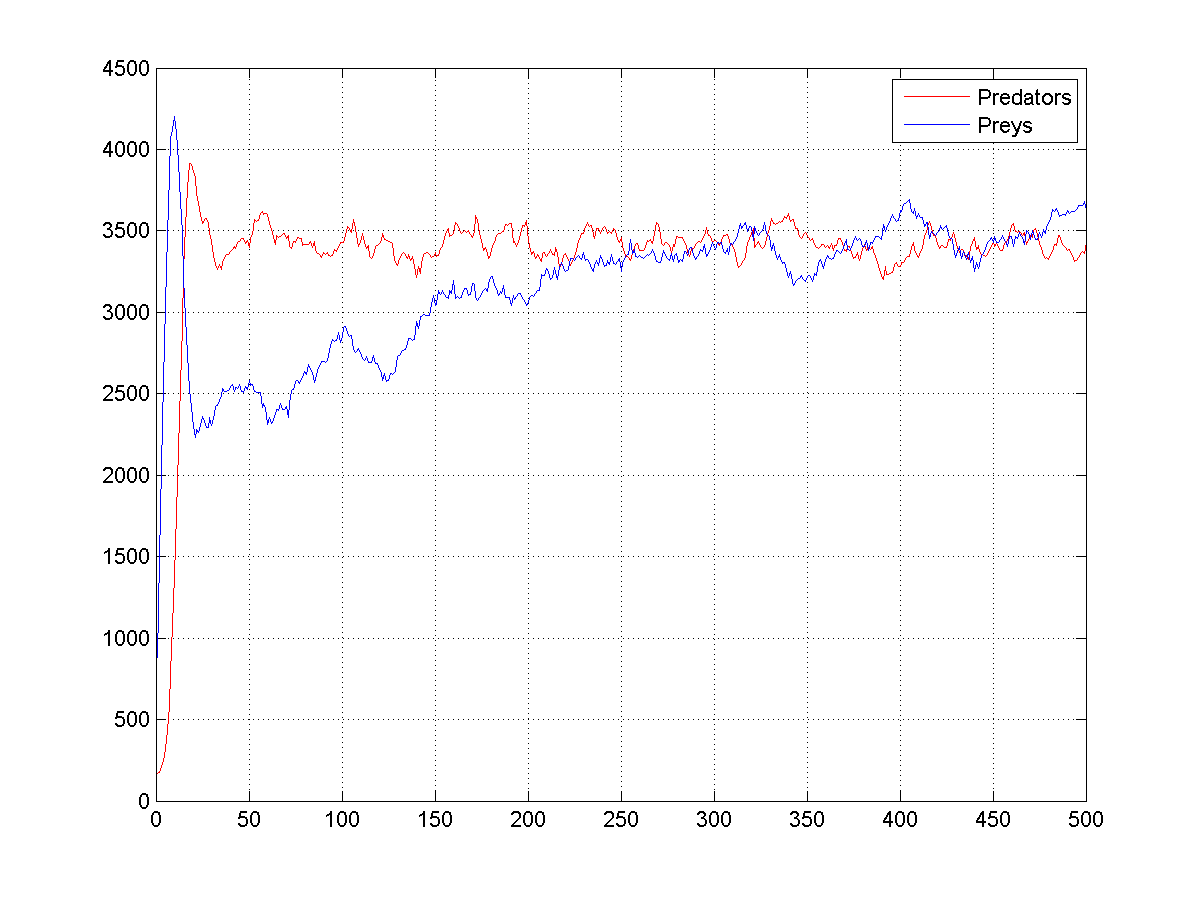
\includegraphics[width=250pt,height=220pt]{figures/2LevelImage.png}
\caption{Predators vs Preys population through time}
\end{figure}
}

\frame{\frametitle{2 Levels Niche}
\begin{figure}[hbtp]
\centering
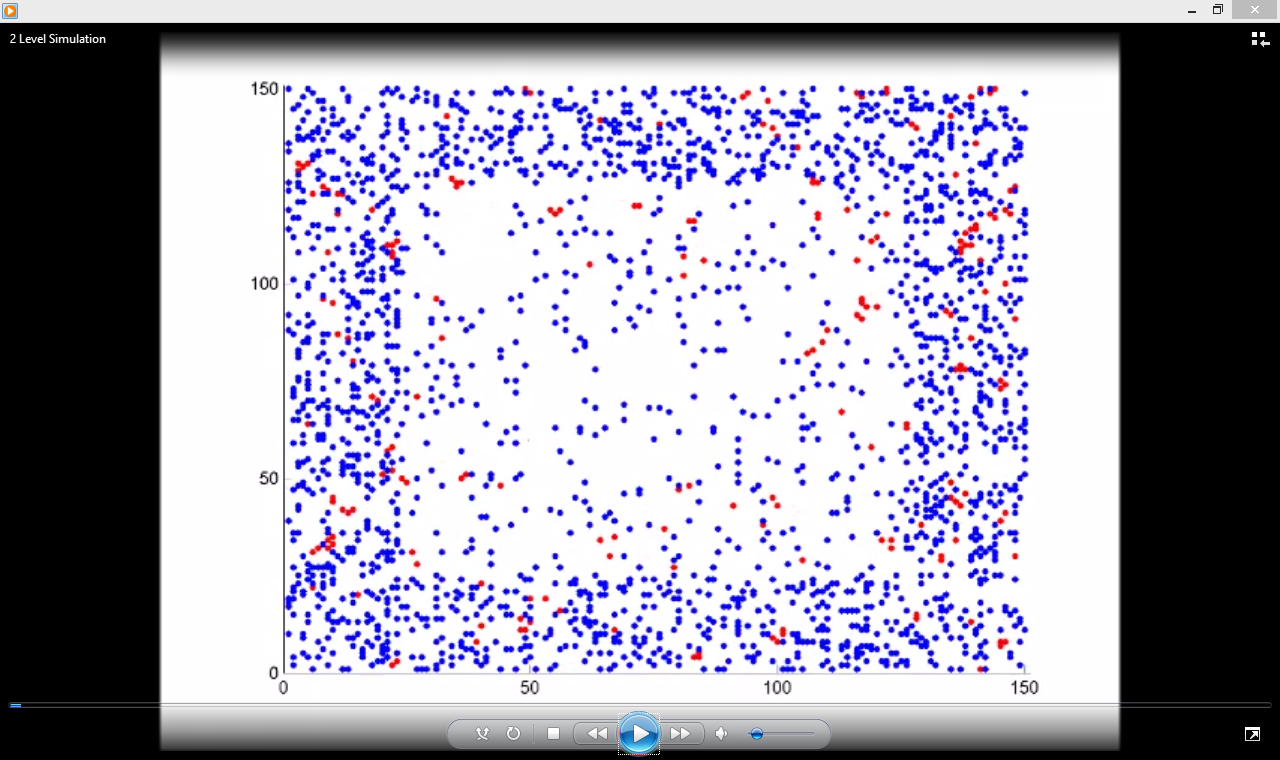
\includegraphics[width=250pt,height=190pt]{figures/2LevelVideo.png}
\end{figure}
}

\section{Comparison}
\subsection{Average Survival Time}
\frame{\frametitle{Average Survival Time}
For each of the 3 variants presented a a simulation of 500 runs was conducted and the 
Mean survival time was observed in terms of iterations
    \begin{table}[!t]
    \tiny
    \renewcommand{\arraystretch}{1}
    \centering
    \begin{tabular}{cccc}
    \hline
    Train/Validate (regions) & \textbf{Mean} & \textbf{Variance}      & \textbf{Median}    \\\hline    
    \textbf{Simple Simulation}     &  98     &  1.4 e+04          & 40.7           \\\hline
    \textbf{Simple Simulation  with predators}     &  40.33     & 8.74          &  39.7063 \\\hline
    \textbf{Niche Simulation}     & 24.11     & 0.1585          & 24.14      \\\hline
        \textbf{2 Level Simulation}     & 3.7309     & 0.0016          & 3.7348      \\\hline
    \end{tabular}
    \end{table}
}
\frame{\frametitle{Average Survival Time}
\begin{figure}[hbtp]
\centering
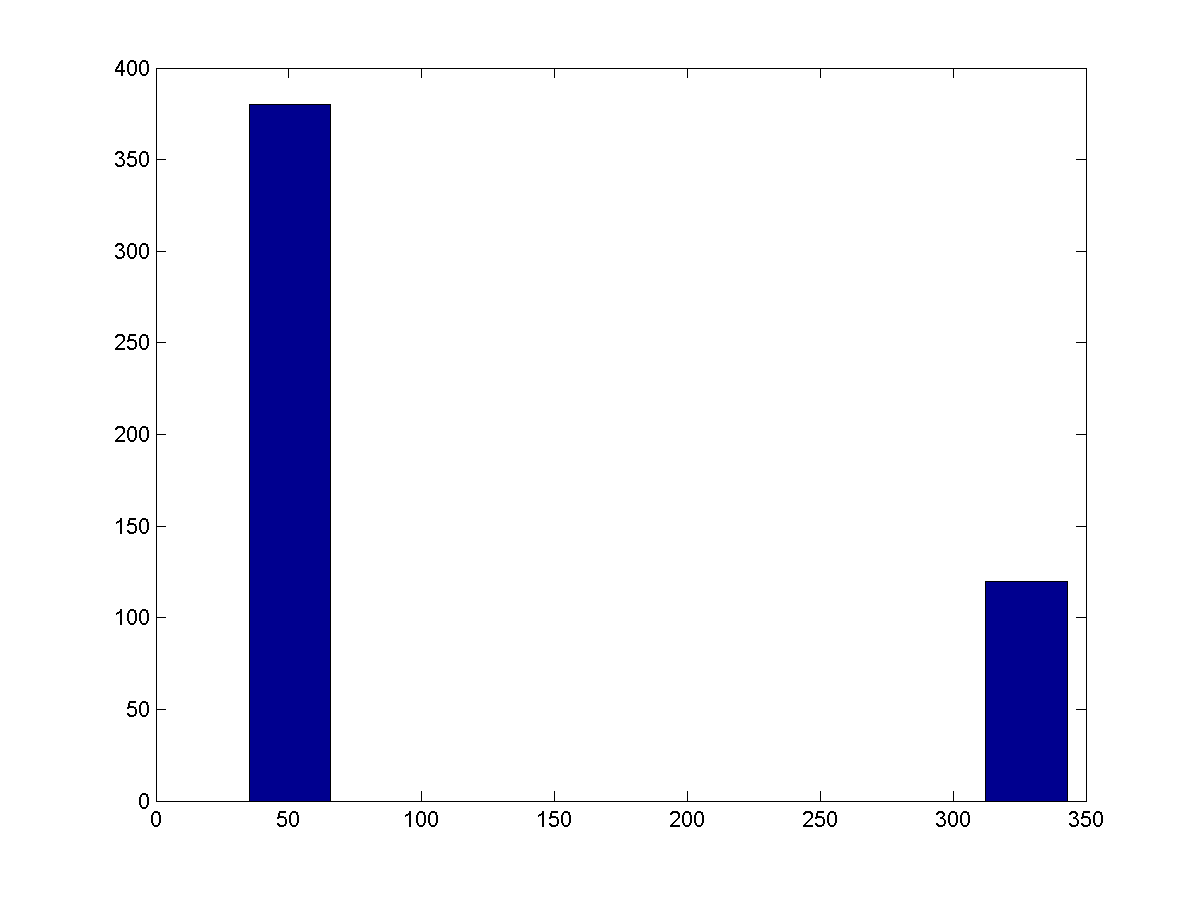
\includegraphics[width=270pt,height=180pt]{figures/histSimple.png}
\caption{Simple simulation Average survival time histogram}
\end{figure}
}

\frame{\frametitle{Average Survival Time}
\begin{figure}[hbtp]
\centering
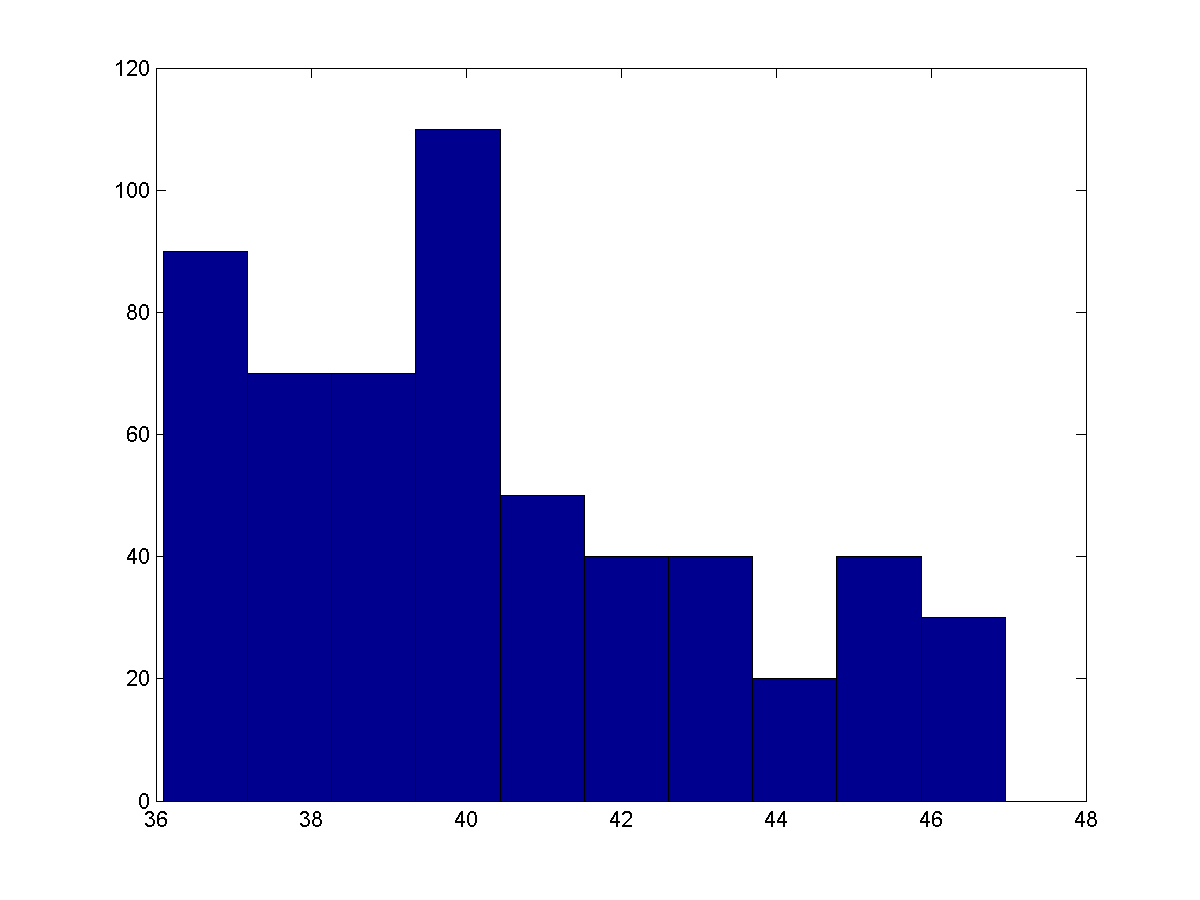
\includegraphics[width=270pt,height=180pt]{figures/SimplNoHist.png}
\caption{Simple with predators Average survival time histogram}
\end{figure}
}

\frame{\frametitle{Average Survival Time}
\begin{figure}[hbtp]
\centering
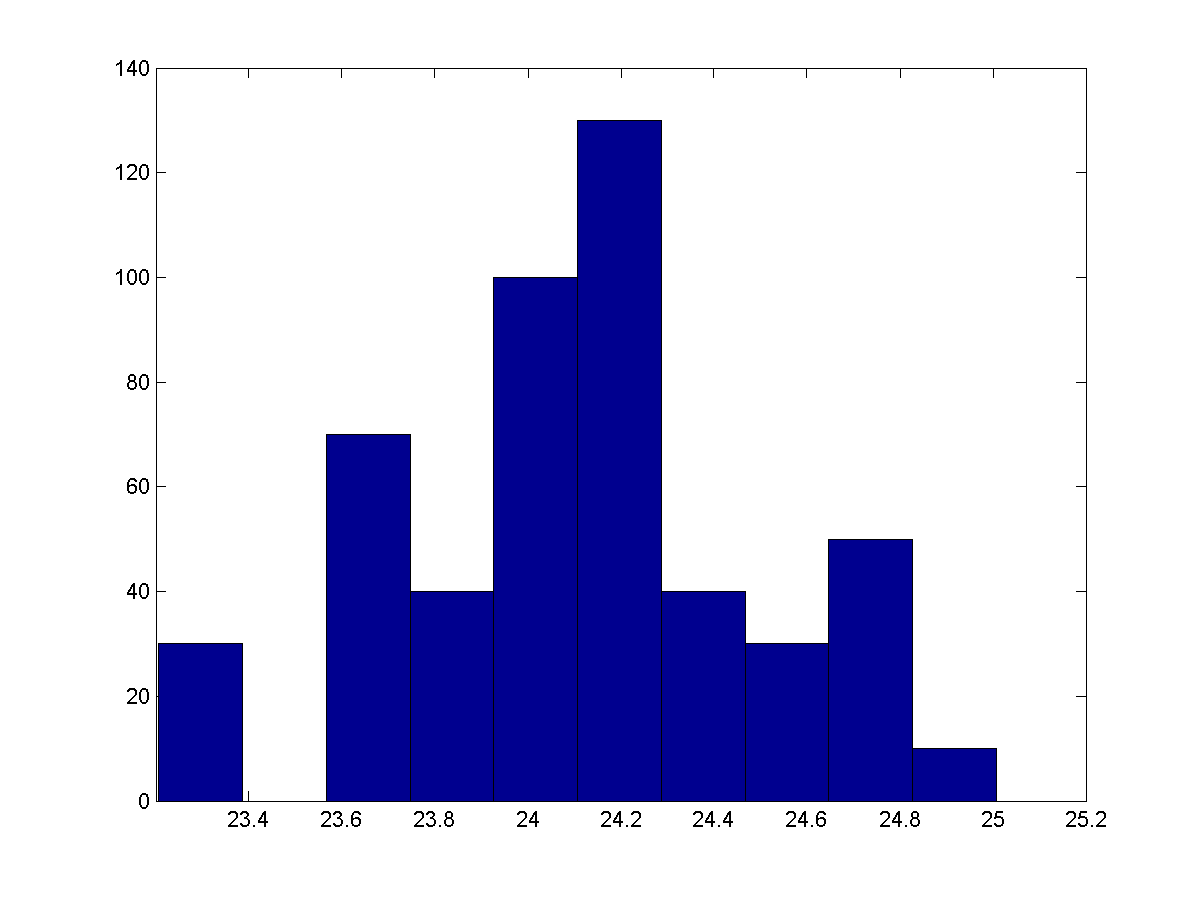
\includegraphics[width=270pt,height=180pt]{figures/NicheHist.png}
\caption{Niche Average survival time histogram}
\end{figure}
}
\frame{\frametitle{Average Survival Time}
\begin{figure}[hbtp]
\centering
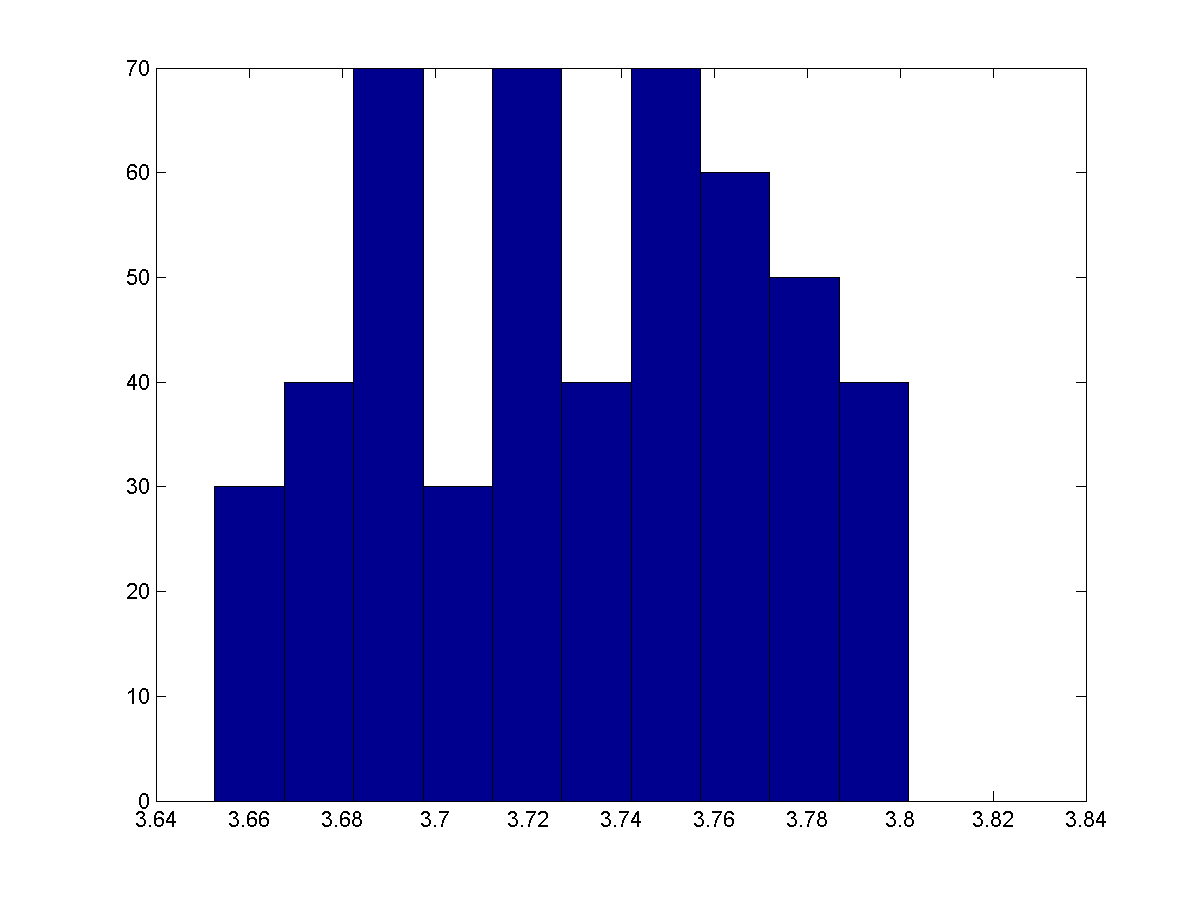
\includegraphics[width=270pt,height=180pt]{figures/2LevelHist.png}
\caption{2 Level Average survival time histogram}
\end{figure}
}
\section*{}
\frame{
    \begin{center}
        \huge
        This is the last slide.\\ 
        \vspace{1cm}
        Any questions?
    \end{center}
}

\frame{\frametitle{References}
\begin{itemize}
\item The Predator-Prey Equations Model : Pennsylvania State University Mathematics Department : http://www.math.psu.edu/tseng/class/Math251/Notes-Predator-Prey.pdf
\item Cellular Automaton :http://mathworld.wolfram.com/CellularAutomaton.html
\item Chapter 12 \& 15 of the lectures
\end{itemize}
}
\end{document} 